%49
\subsection{Elemek eltávolítása a sorból (dequeue)}
\begin{frame}
  \begin{columns}[c]
    \column{0.52\textwidth}
      \scriptsize
      \begin{exampleblock}{\textattachfile{sor2.cpp}{sor2.cpp}}
        \scriptsize
        \lstinputlisting[style=cpp,linerange={26-41},numbers=left,firstnumber=26]{sor2.cpp}
      \end{exampleblock}
    \column{0.43\textwidth}
      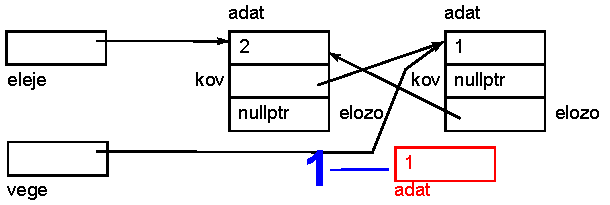
\includegraphics[width=\textwidth]{sor/sor20.pdf}
  \end{columns}
\end{frame}

%50
\begin{frame}
  \begin{columns}[c]
    \column{0.52\textwidth}
      \scriptsize
      \begin{exampleblock}{\textattachfile{sor2.cpp}{sor2.cpp}}
        \scriptsize
        \lstinputlisting[style=cpp,linerange={26-41},numbers=left,firstnumber=26]{sor2.cpp}
      \end{exampleblock}
    \column{0.43\textwidth}
      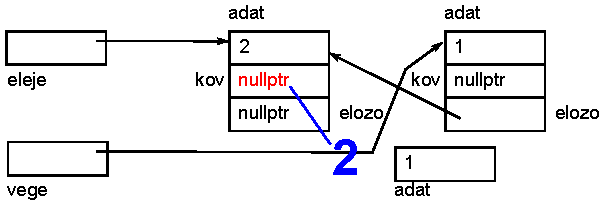
\includegraphics[width=\textwidth]{sor/sor21.pdf}
  \end{columns}
\end{frame}

%51
\begin{frame}
  \begin{columns}[c]
    \column{0.52\textwidth}
      \scriptsize
      \begin{exampleblock}{\textattachfile{sor2.cpp}{sor2.cpp}}
        \scriptsize
        \lstinputlisting[style=cpp,linerange={26-41},numbers=left,firstnumber=26]{sor2.cpp}
      \end{exampleblock}
    \column{0.43\textwidth}
      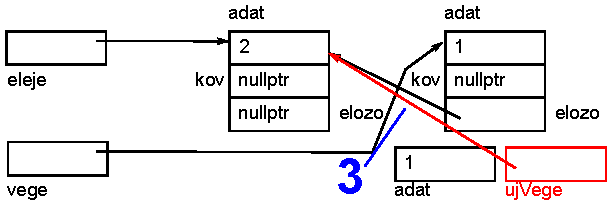
\includegraphics[width=\textwidth]{sor/sor22.pdf}
  \end{columns}
\end{frame}

%52
\begin{frame}
  \begin{columns}[c]
    \column{0.52\textwidth}
      \scriptsize
      \begin{exampleblock}{\textattachfile{sor2.cpp}{sor2.cpp}}
        \scriptsize
        \lstinputlisting[style=cpp,linerange={26-41},numbers=left,firstnumber=26]{sor2.cpp}
      \end{exampleblock}
    \column{0.43\textwidth}
      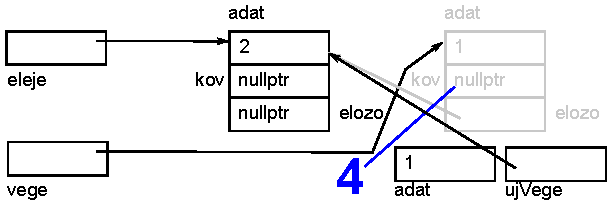
\includegraphics[width=\textwidth]{sor/sor23.pdf}
  \end{columns}
\end{frame}

%53
\begin{frame}
  \begin{columns}[c]
    \column{0.52\textwidth}
      \scriptsize
      \begin{exampleblock}{\textattachfile{sor2.cpp}{sor2.cpp}}
        \scriptsize
        \lstinputlisting[style=cpp,linerange={26-41},numbers=left,firstnumber=26]{sor2.cpp}
      \end{exampleblock}
    \column{0.43\textwidth}
      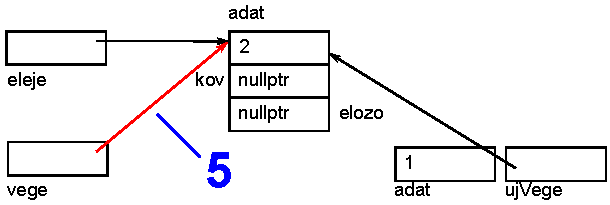
\includegraphics[width=\textwidth]{sor/sor24.pdf}
  \end{columns}
\end{frame}

%54
\begin{frame}
  \begin{columns}[c]
    \column{0.52\textwidth}
      \scriptsize
      \begin{exampleblock}{\textattachfile{sor2.cpp}{sor2.cpp}}
        \scriptsize
        \lstinputlisting[style=cpp,linerange={26-41},numbers=left,firstnumber=26]{sor2.cpp}
      \end{exampleblock}
    \column{0.43\textwidth}
      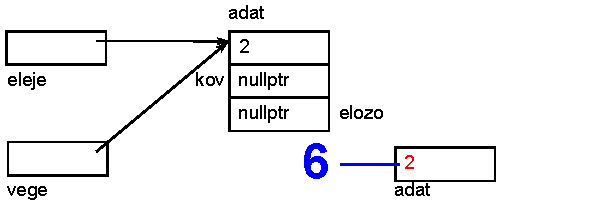
\includegraphics[width=\textwidth]{sor/sor25.pdf}
  \end{columns}
\end{frame}

%55
\begin{frame}
  \begin{columns}[c]
    \column{0.52\textwidth}
      \scriptsize
      \begin{exampleblock}{\textattachfile{sor2.cpp}{sor2.cpp}}
        \scriptsize
        \lstinputlisting[style=cpp,linerange={26-41},numbers=left,firstnumber=26]{sor2.cpp}
      \end{exampleblock}
    \column{0.43\textwidth}
      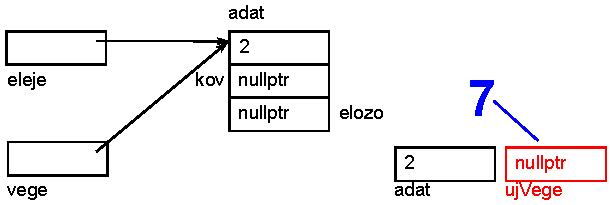
\includegraphics[width=\textwidth]{sor/sor26.pdf}
  \end{columns}
\end{frame}

%56
\begin{frame}
  \begin{columns}[c]
    \column{0.52\textwidth}
      \scriptsize
      \begin{exampleblock}{\textattachfile{sor2.cpp}{sor2.cpp}}
        \scriptsize
        \lstinputlisting[style=cpp,linerange={26-41},numbers=left,firstnumber=26]{sor2.cpp}
      \end{exampleblock}
    \column{0.43\textwidth}
      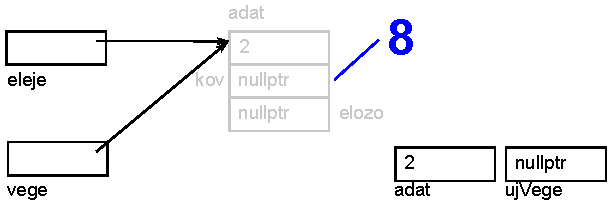
\includegraphics[width=\textwidth]{sor/sor27.pdf}
  \end{columns}
\end{frame}

%57
\begin{frame}
  \begin{columns}[c]
    \column{0.52\textwidth}
      \scriptsize
      \begin{exampleblock}{\textattachfile{sor2.cpp}{sor2.cpp}}
        \scriptsize
        \lstinputlisting[style=cpp,linerange={26-41},numbers=left,firstnumber=26]{sor2.cpp}
      \end{exampleblock}
    \column{0.43\textwidth}
      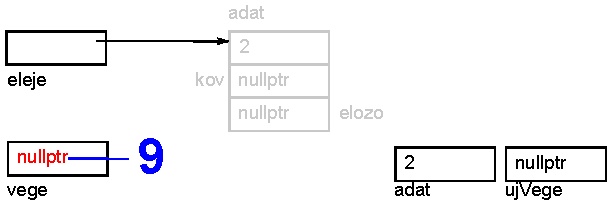
\includegraphics[width=\textwidth]{sor/sor28.pdf}
  \end{columns}
\end{frame}

%58
\begin{frame}
  \begin{columns}[c]
    \column{0.52\textwidth}
      \scriptsize
      \begin{exampleblock}{\textattachfile{sor2.cpp}{sor2.cpp}}
        \scriptsize
        \lstinputlisting[style=cpp,linerange={26-41},numbers=left,firstnumber=26]{sor2.cpp}
      \end{exampleblock}
    \column{0.43\textwidth}
      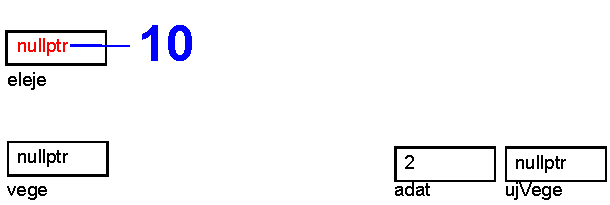
\includegraphics[width=\textwidth]{sor/sor29.pdf}
  \end{columns}
\end{frame}